% Order-preserving PathMap byte keys for PageAddress::to_key().
% Tag bytes order the space (corpus 0x01..0x04 < scratch 0x10); integer fields
% are sign-flipped big-endian so lexicographic byte order == numeric order.
% Drawn in pure TikZ (one cell = one byte) for full colour control.
\documentclass[border=8pt]{standalone}
\usepackage{tikz}
\usepackage{xcolor}
\definecolor{tagc}{HTML}{DC2626}
\definecolor{idc}{HTML}{4F46E5}
\definecolor{spanc}{HTML}{0D9488}
\definecolor{treec}{HTML}{7C3AED}
\definecolor{slotc}{HTML}{D97706}
\begin{document}
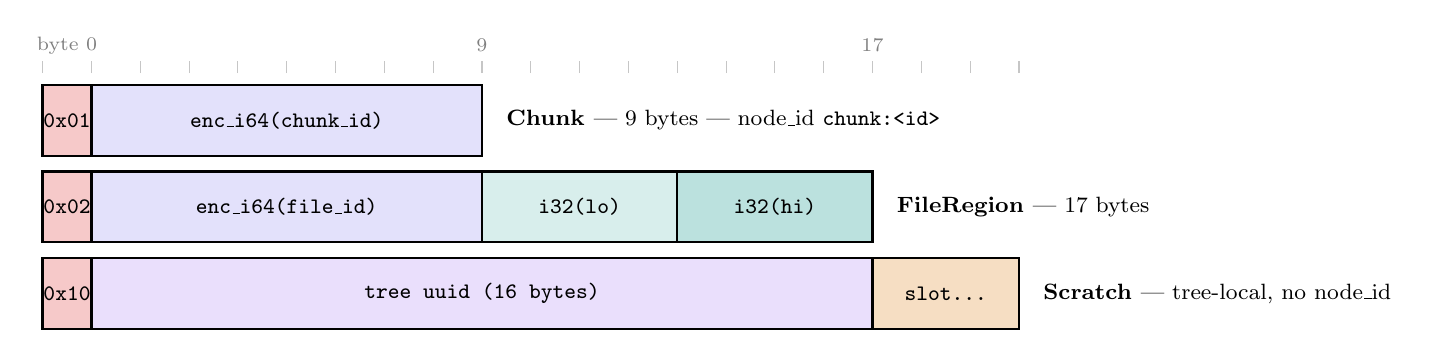
\begin{tikzpicture}[x=0.62cm, y=1cm, font=\sffamily]
  \tikzset{lab/.style={anchor=west, font=\footnotesize\bfseries}}
  % byte ruler
  \foreach \x in {0,1,...,20} { \draw[gray!45] (\x,3.05) -- (\x,3.2); }
  \node[font=\scriptsize, gray] at (0.5,3.4) {byte 0};
  \node[font=\scriptsize, gray] at (9,3.4) {9};
  \node[font=\scriptsize, gray] at (17,3.4) {17};

  % Row 1 — Chunk (9 bytes)
  \fill[tagc!25] (0,2) rectangle (1,2.9);  \draw[thick] (0,2) rectangle (1,2.9);
  \node[font=\ttfamily\footnotesize] at (0.5,2.45) {0x01};
  \fill[idc!16] (1,2) rectangle (9,2.9);   \draw[thick] (1,2) rectangle (9,2.9);
  \node[font=\ttfamily\footnotesize] at (5,2.45) {enc\_i64(chunk\_id)};
  \node[lab] at (9.3,2.45) {Chunk \textmd{— 9 bytes — node\_id \ttfamily chunk:<id>}};

  % Row 2 — FileRegion (17 bytes)
  \fill[tagc!25] (0,0.9) rectangle (1,1.8);  \draw[thick] (0,0.9) rectangle (1,1.8);
  \node[font=\ttfamily\footnotesize] at (0.5,1.35) {0x02};
  \fill[idc!16] (1,0.9) rectangle (9,1.8);   \draw[thick] (1,0.9) rectangle (9,1.8);
  \node[font=\ttfamily\footnotesize] at (5,1.35) {enc\_i64(file\_id)};
  \fill[spanc!16] (9,0.9) rectangle (13,1.8);  \draw[thick] (9,0.9) rectangle (13,1.8);
  \node[font=\ttfamily\footnotesize] at (11,1.35) {i32(lo)};
  \fill[spanc!28] (13,0.9) rectangle (17,1.8); \draw[thick] (13,0.9) rectangle (17,1.8);
  \node[font=\ttfamily\footnotesize] at (15,1.35) {i32(hi)};
  \node[lab] at (17.3,1.35) {FileRegion \textmd{— 17 bytes}};

  % Row 3 — Scratch (1 + 16 + n)
  \fill[tagc!25] (0,-0.2) rectangle (1,0.7);  \draw[thick] (0,-0.2) rectangle (1,0.7);
  \node[font=\ttfamily\footnotesize] at (0.5,0.25) {0x10};
  \fill[treec!16] (1,-0.2) rectangle (17,0.7); \draw[thick] (1,-0.2) rectangle (17,0.7);
  \node[font=\ttfamily\footnotesize] at (9,0.25) {tree uuid (16 bytes)};
  \fill[slotc!24] (17,-0.2) rectangle (20,0.7); \draw[thick] (17,-0.2) rectangle (20,0.7);
  \node[font=\ttfamily\footnotesize] at (18.5,0.25) {slot…};
  \node[lab] at (20.3,0.25) {Scratch \textmd{— tree-local, no node\_id}};
\end{tikzpicture}
\end{document}
